\subsection{Biological insight}
\subsubsection{IUT Component}
At the IUT component, both SigNet and MARINa deliver us with a list of seeds which we can use as a start point to initiate research. We get a ranked list of nodes which are potentially the most influent upstream individuals.
\\

\begin{figure}[!h]
    \centering
    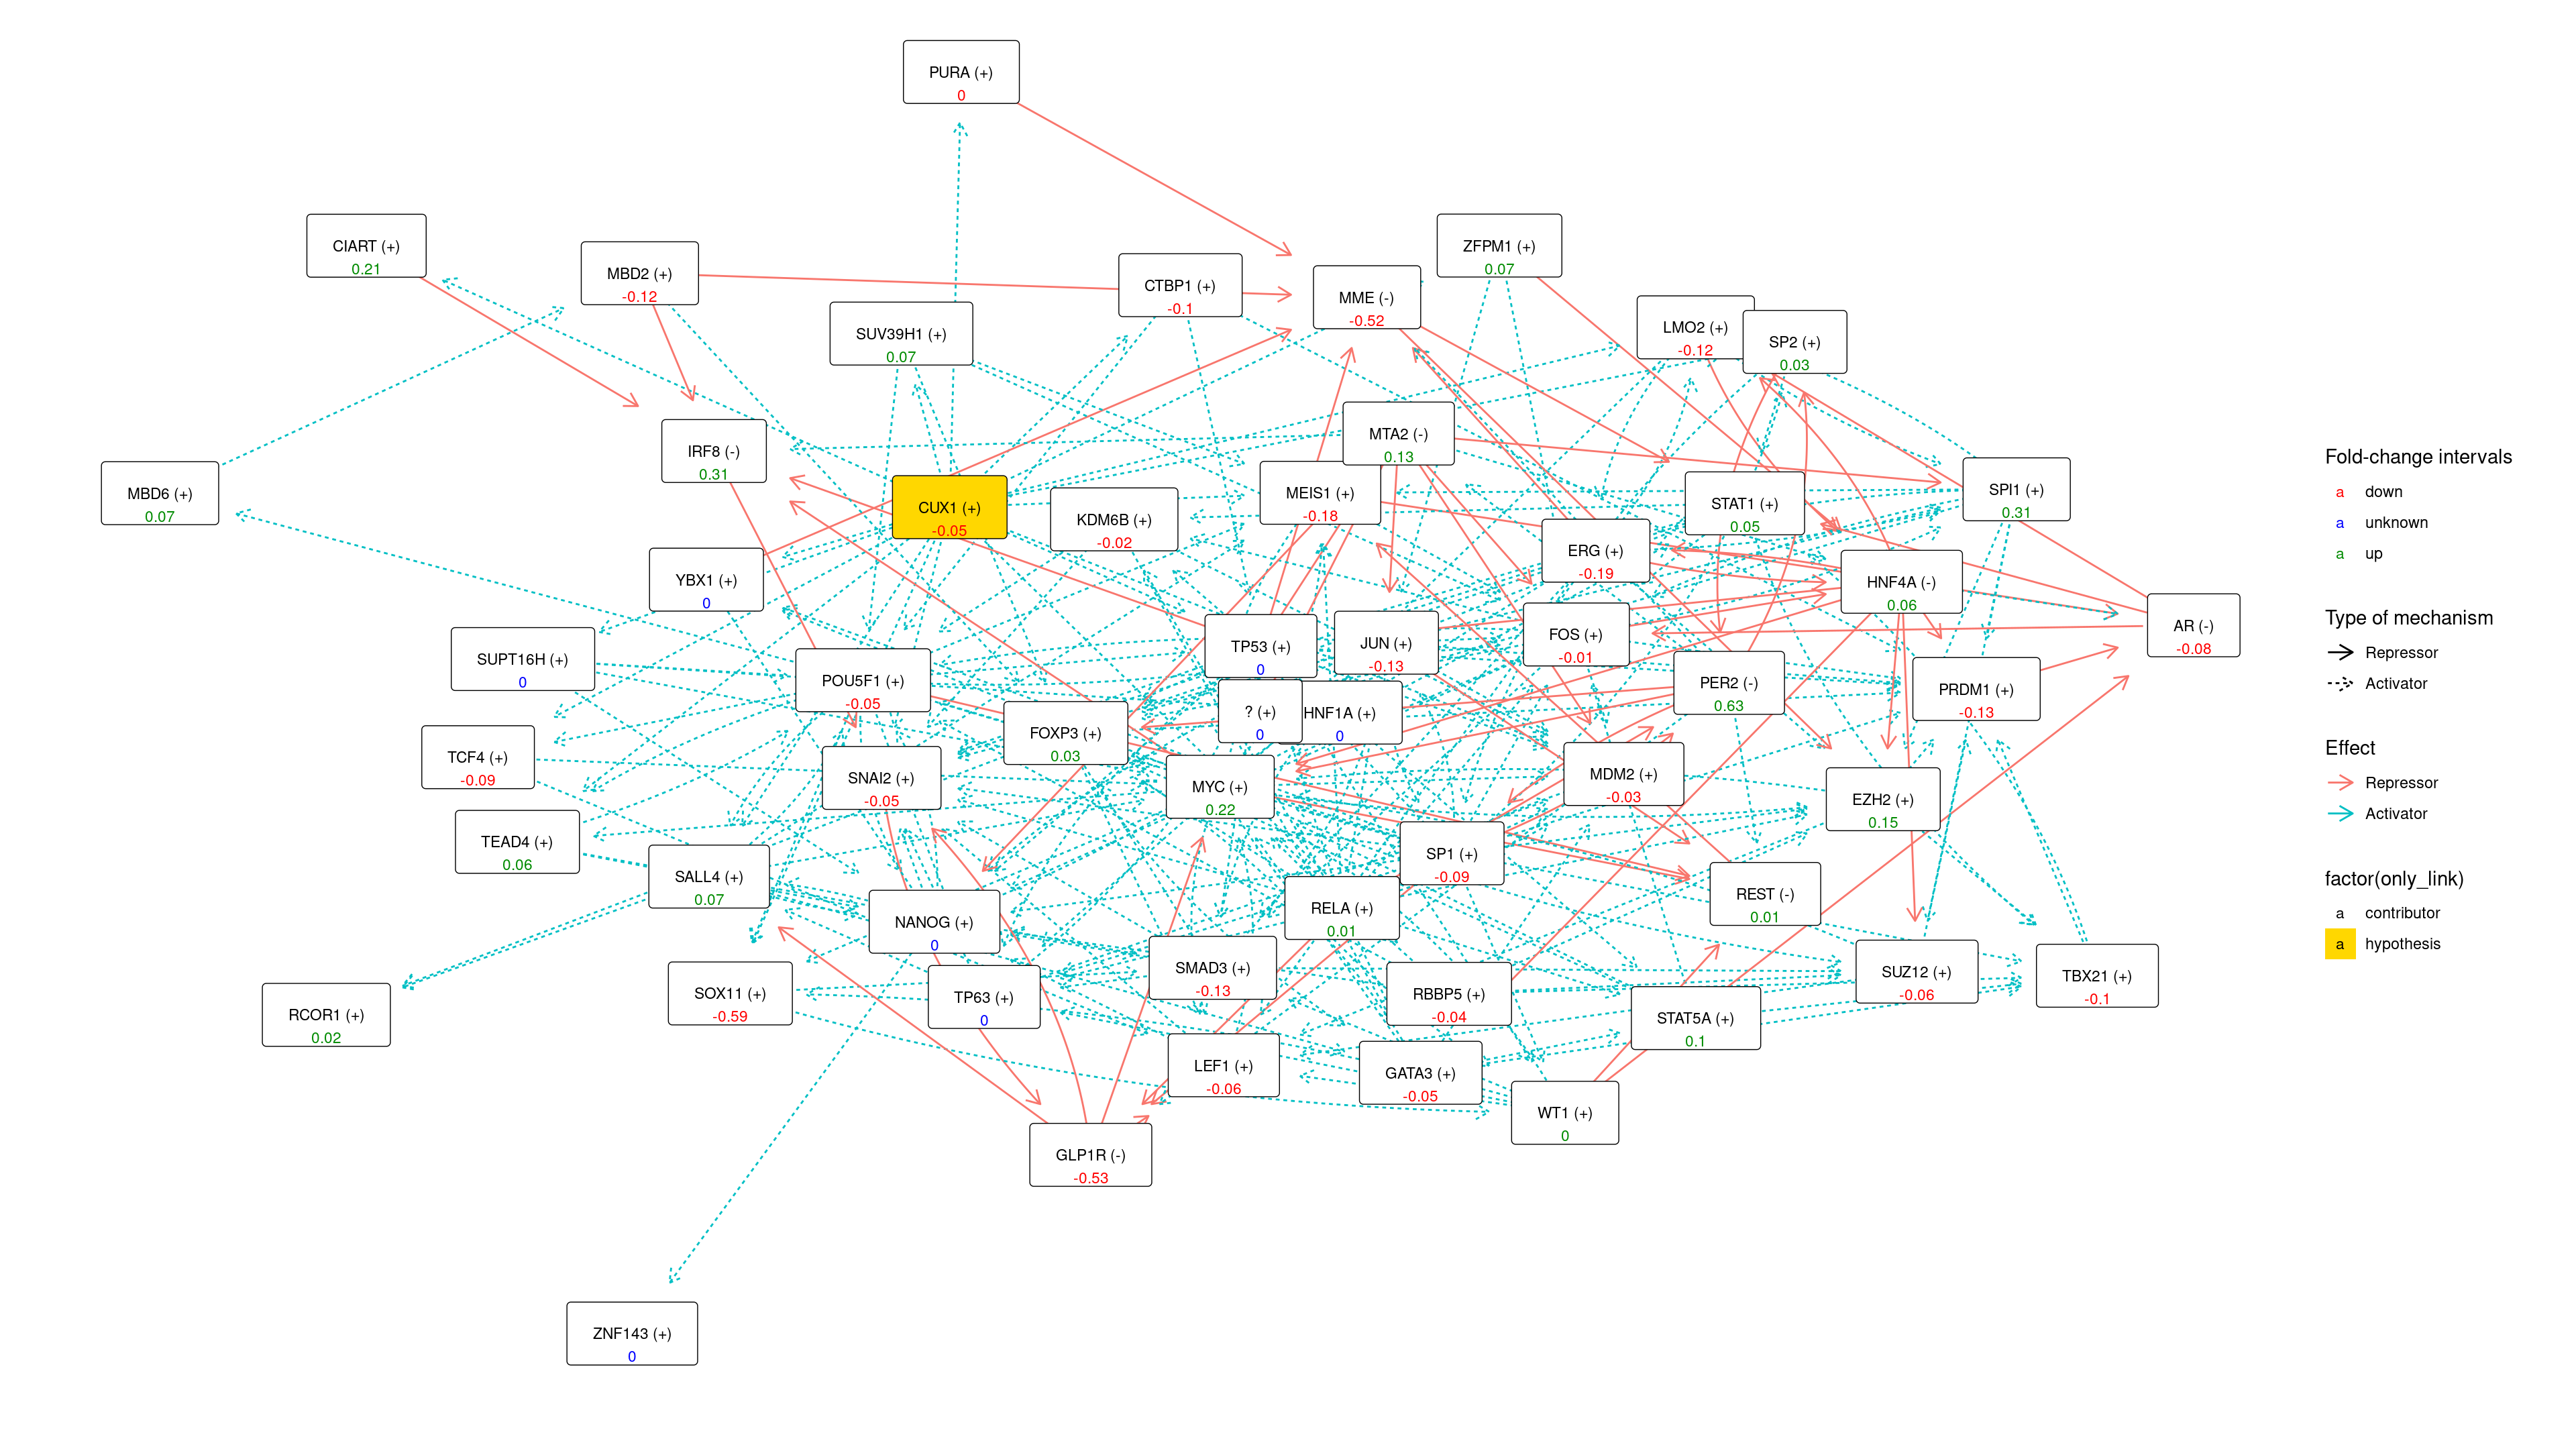
\includegraphics[width=\textwidth, height=\textheight, keepaspectratio]{Major Thesis/figures/iut/graph/SWITCH4m50-CUX1.png}
    \caption{Interaction sub-network of the top DE ranked gene CUX1 (Cut Like Homeobox 1) at node 50\% contribution. SigNet run on Switch 4m contrast. Each node include its original fold-change, coloured to aid visualization.}
    \label{fig:graph-expansion}
\end{figure}

An observation of the system for the specific SWITCH 4m contrast is displayed in Figure \ref{fig:graph-expansion}, where interactions for the top DE gene has been retrieved, keeping only the 50\% of the nodes that contributed to its rank rise. In this particular result, we aim to investigate the surroundings and inner interactions of CUX1. Its product is known to have a gene regulatory purpose and influence on the cell cycle. More precisely its down-regulation has been related to tumorigenesis \cite{Wong2014InactivatingTumorigenesis}.


Besides, CUX1 belongs to the top 10 ranked for SigNet in all contrasts that involve cigarette smoke (CS) in any proportion and duration (3R4F, SWITCH, CESS), as shown in Figure \ref{fig:heatmap-overview}. Same happens with RELA Proto-Oncogene (as NF-KB Subunit), MYC Proto-oncogene, where we observe a minor rank divergence.
\\

At first sight, the information retrieved aligns with an expected outcome, i.e. since we are handling lung expression data from smoked and control cases, we anticipate insight lined up with any of the main known problems related to smoking, such as proto-oncogenes supportting lung cancer. However, is on biology experts to determine for which to aim to proceed, keeping divergent solutions as a possible outcome, mainly due to the unpredictability, and hidden mechanistic when it comes to systems biology.
\\

On the other hand, on a broader view of control results, non-smoke contrasts (THS and  CHTP) suffer a more severe cut in the input, as a result of the minimum FC requirement at the Format Core. Smoke contrasts (3R4F, SWITCH and CESS) have more nodes which present DEG than their non-smoke counterparts, i.e. THS and CHTP aerosol only induce low effects in the lung, which are then difficult to link to a specific mechanism. This leaves us with fewer start points to trigger the graph construction.
\\

Entangled static networks such as Figure \ref{fig:graph-expansion} hinder research. Due to this, an interactive version of the graph is offered alongside with the generated PNG graphs. It allows live node interaction through the web browser. A preview of the interactive version and the remaining results across all contrasts can be found in Suppl.Figures \ref{section:suppl:results}.
\\

On the other hand, contrasts exposed to CS dispose of entangled contributor’s graphs. At a cutoff of 50\% of cumulative votes, node count rounded mean is 200 (Figure \ref{fig:compare-density}). For the group which does not have CS exposition, the mean is 5. Based on this data, we conclude the votes and decisive power of all the targets which contribute to hypothesis support in CS contrasts is significantly lower than in non-CS contrasts.
\\

\begin{figure}
    \begin{subfigure}{0.3\linewidth}
        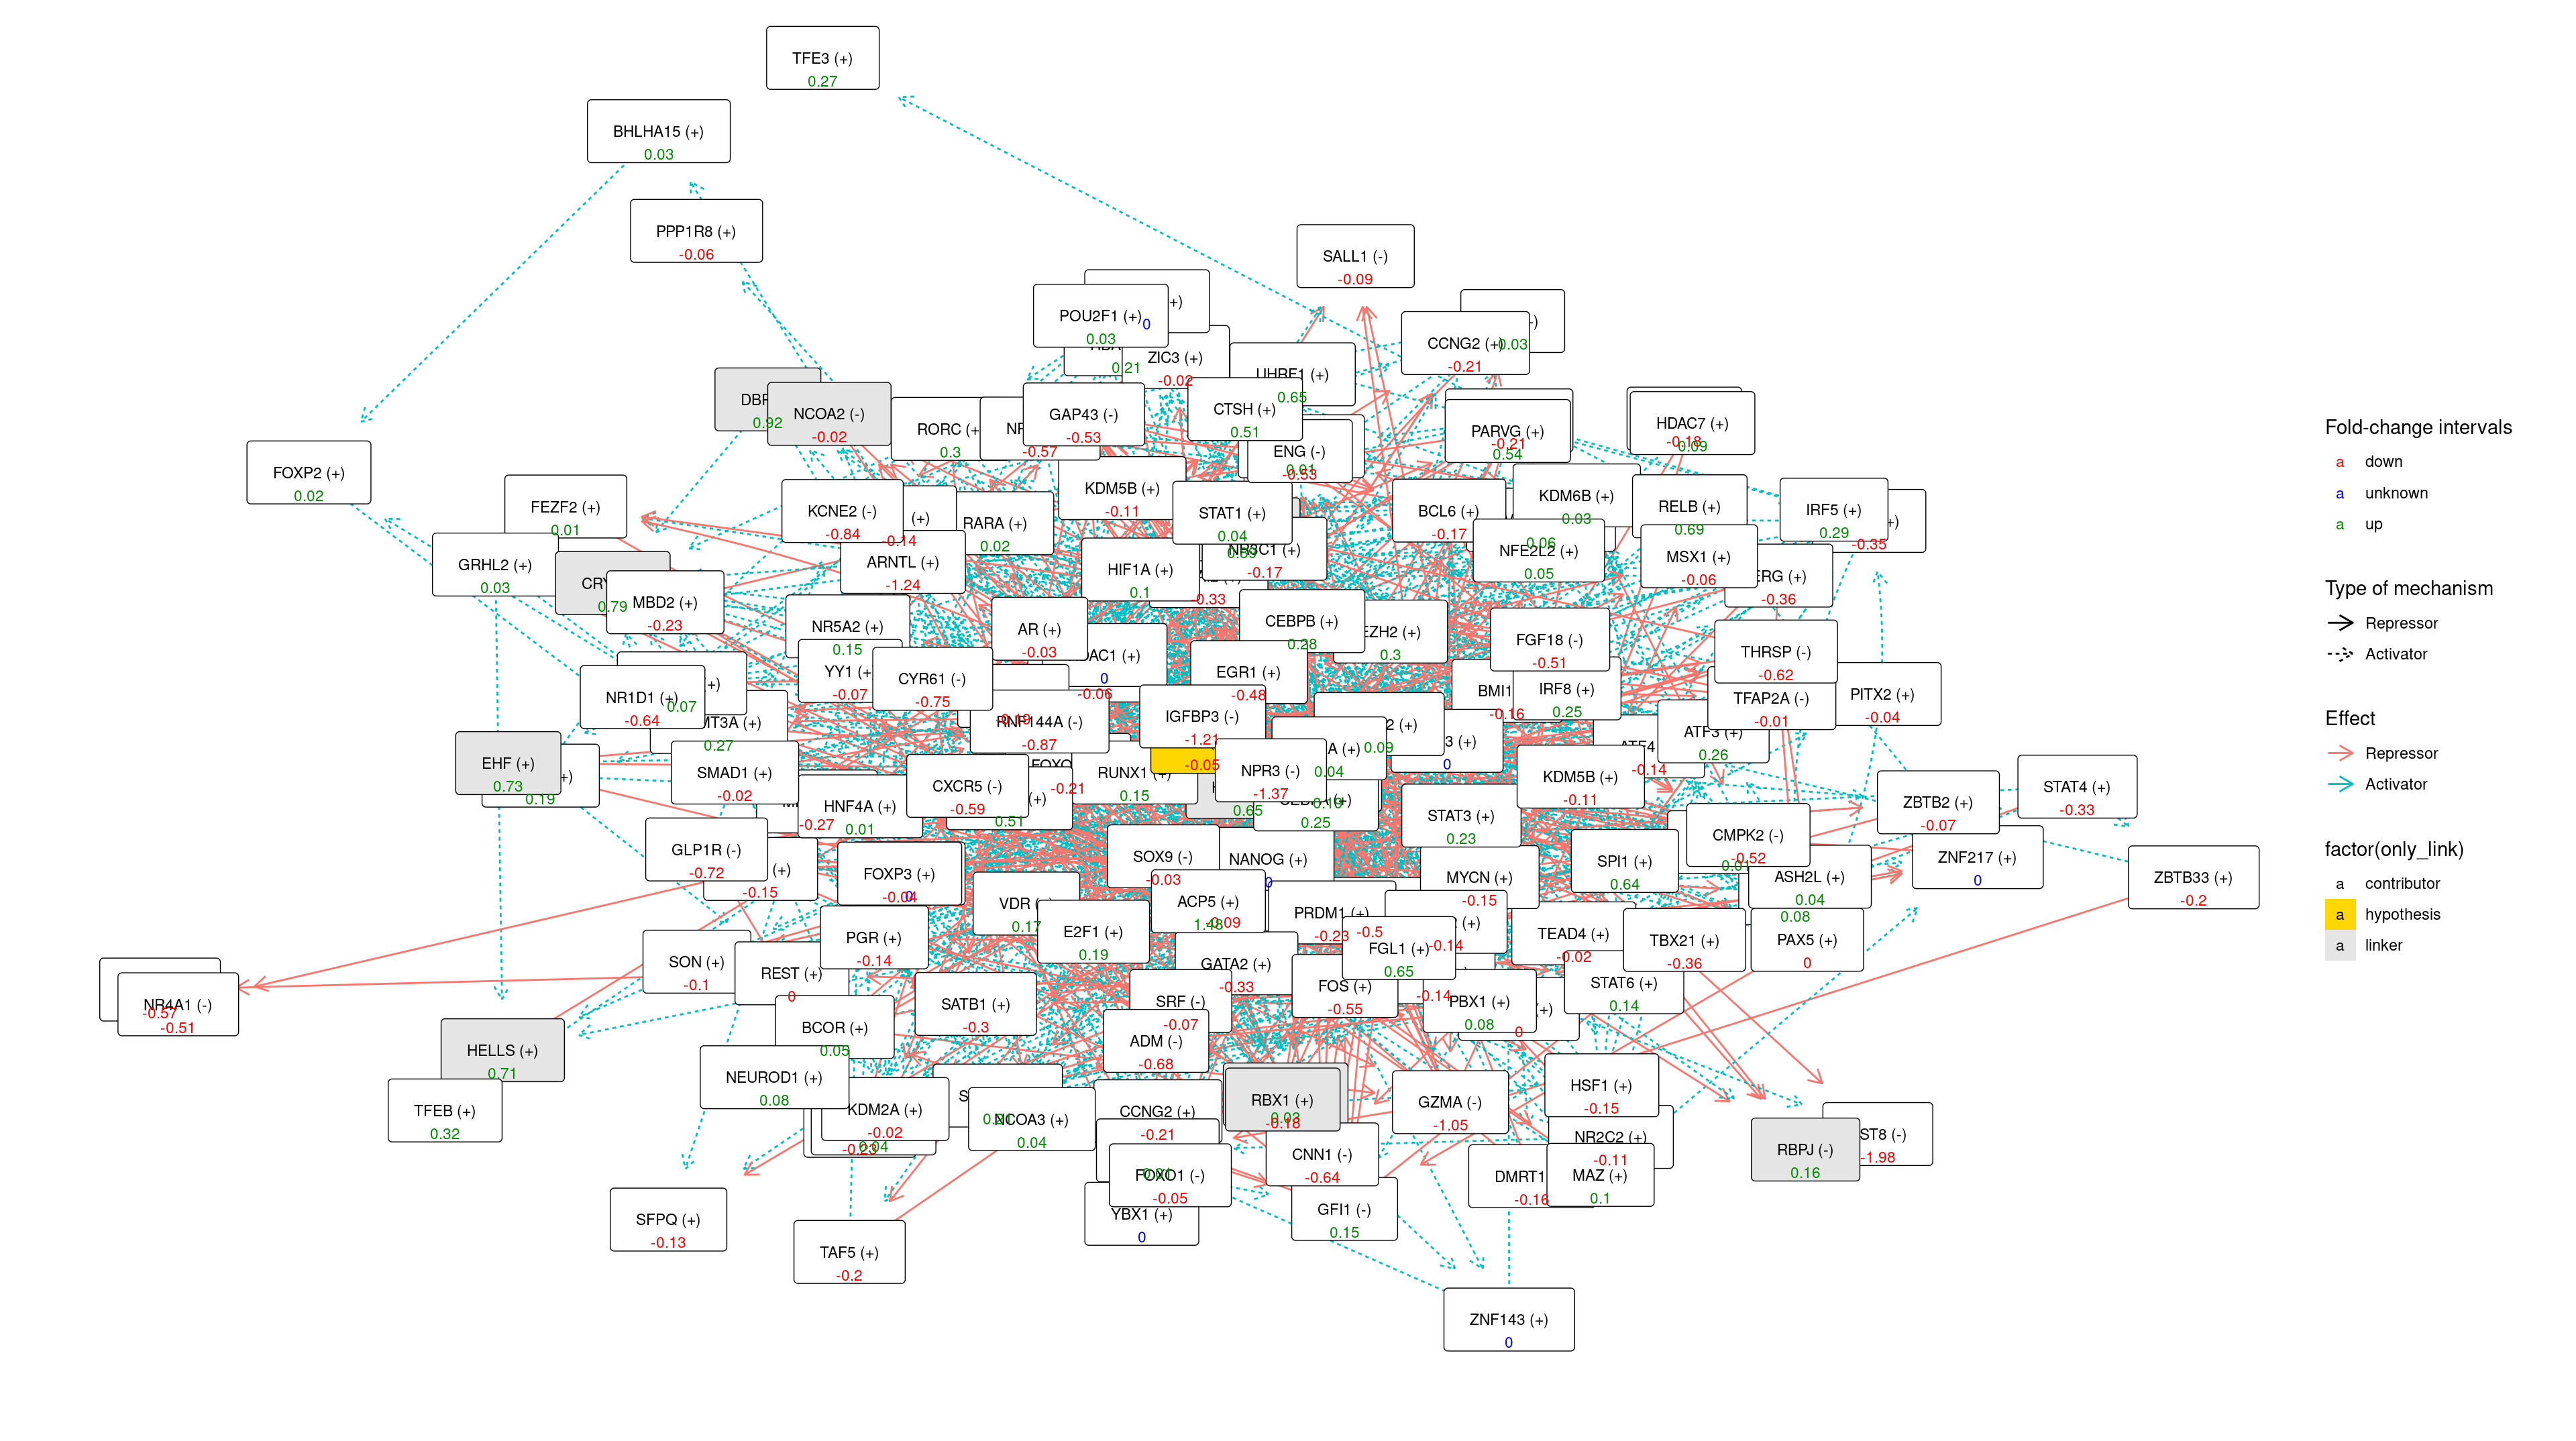
\includegraphics[width=\textwidth, height=\textheight, keepaspectratio]{Major Thesis/figures/iut/graph/3R4F4m50-SP1.png}
            \caption{3R4F 4m contrast}
            \label{img:smoke}
    \end{subfigure}
    \hfill
    \begin{subfigure}{0.3\linewidth}
        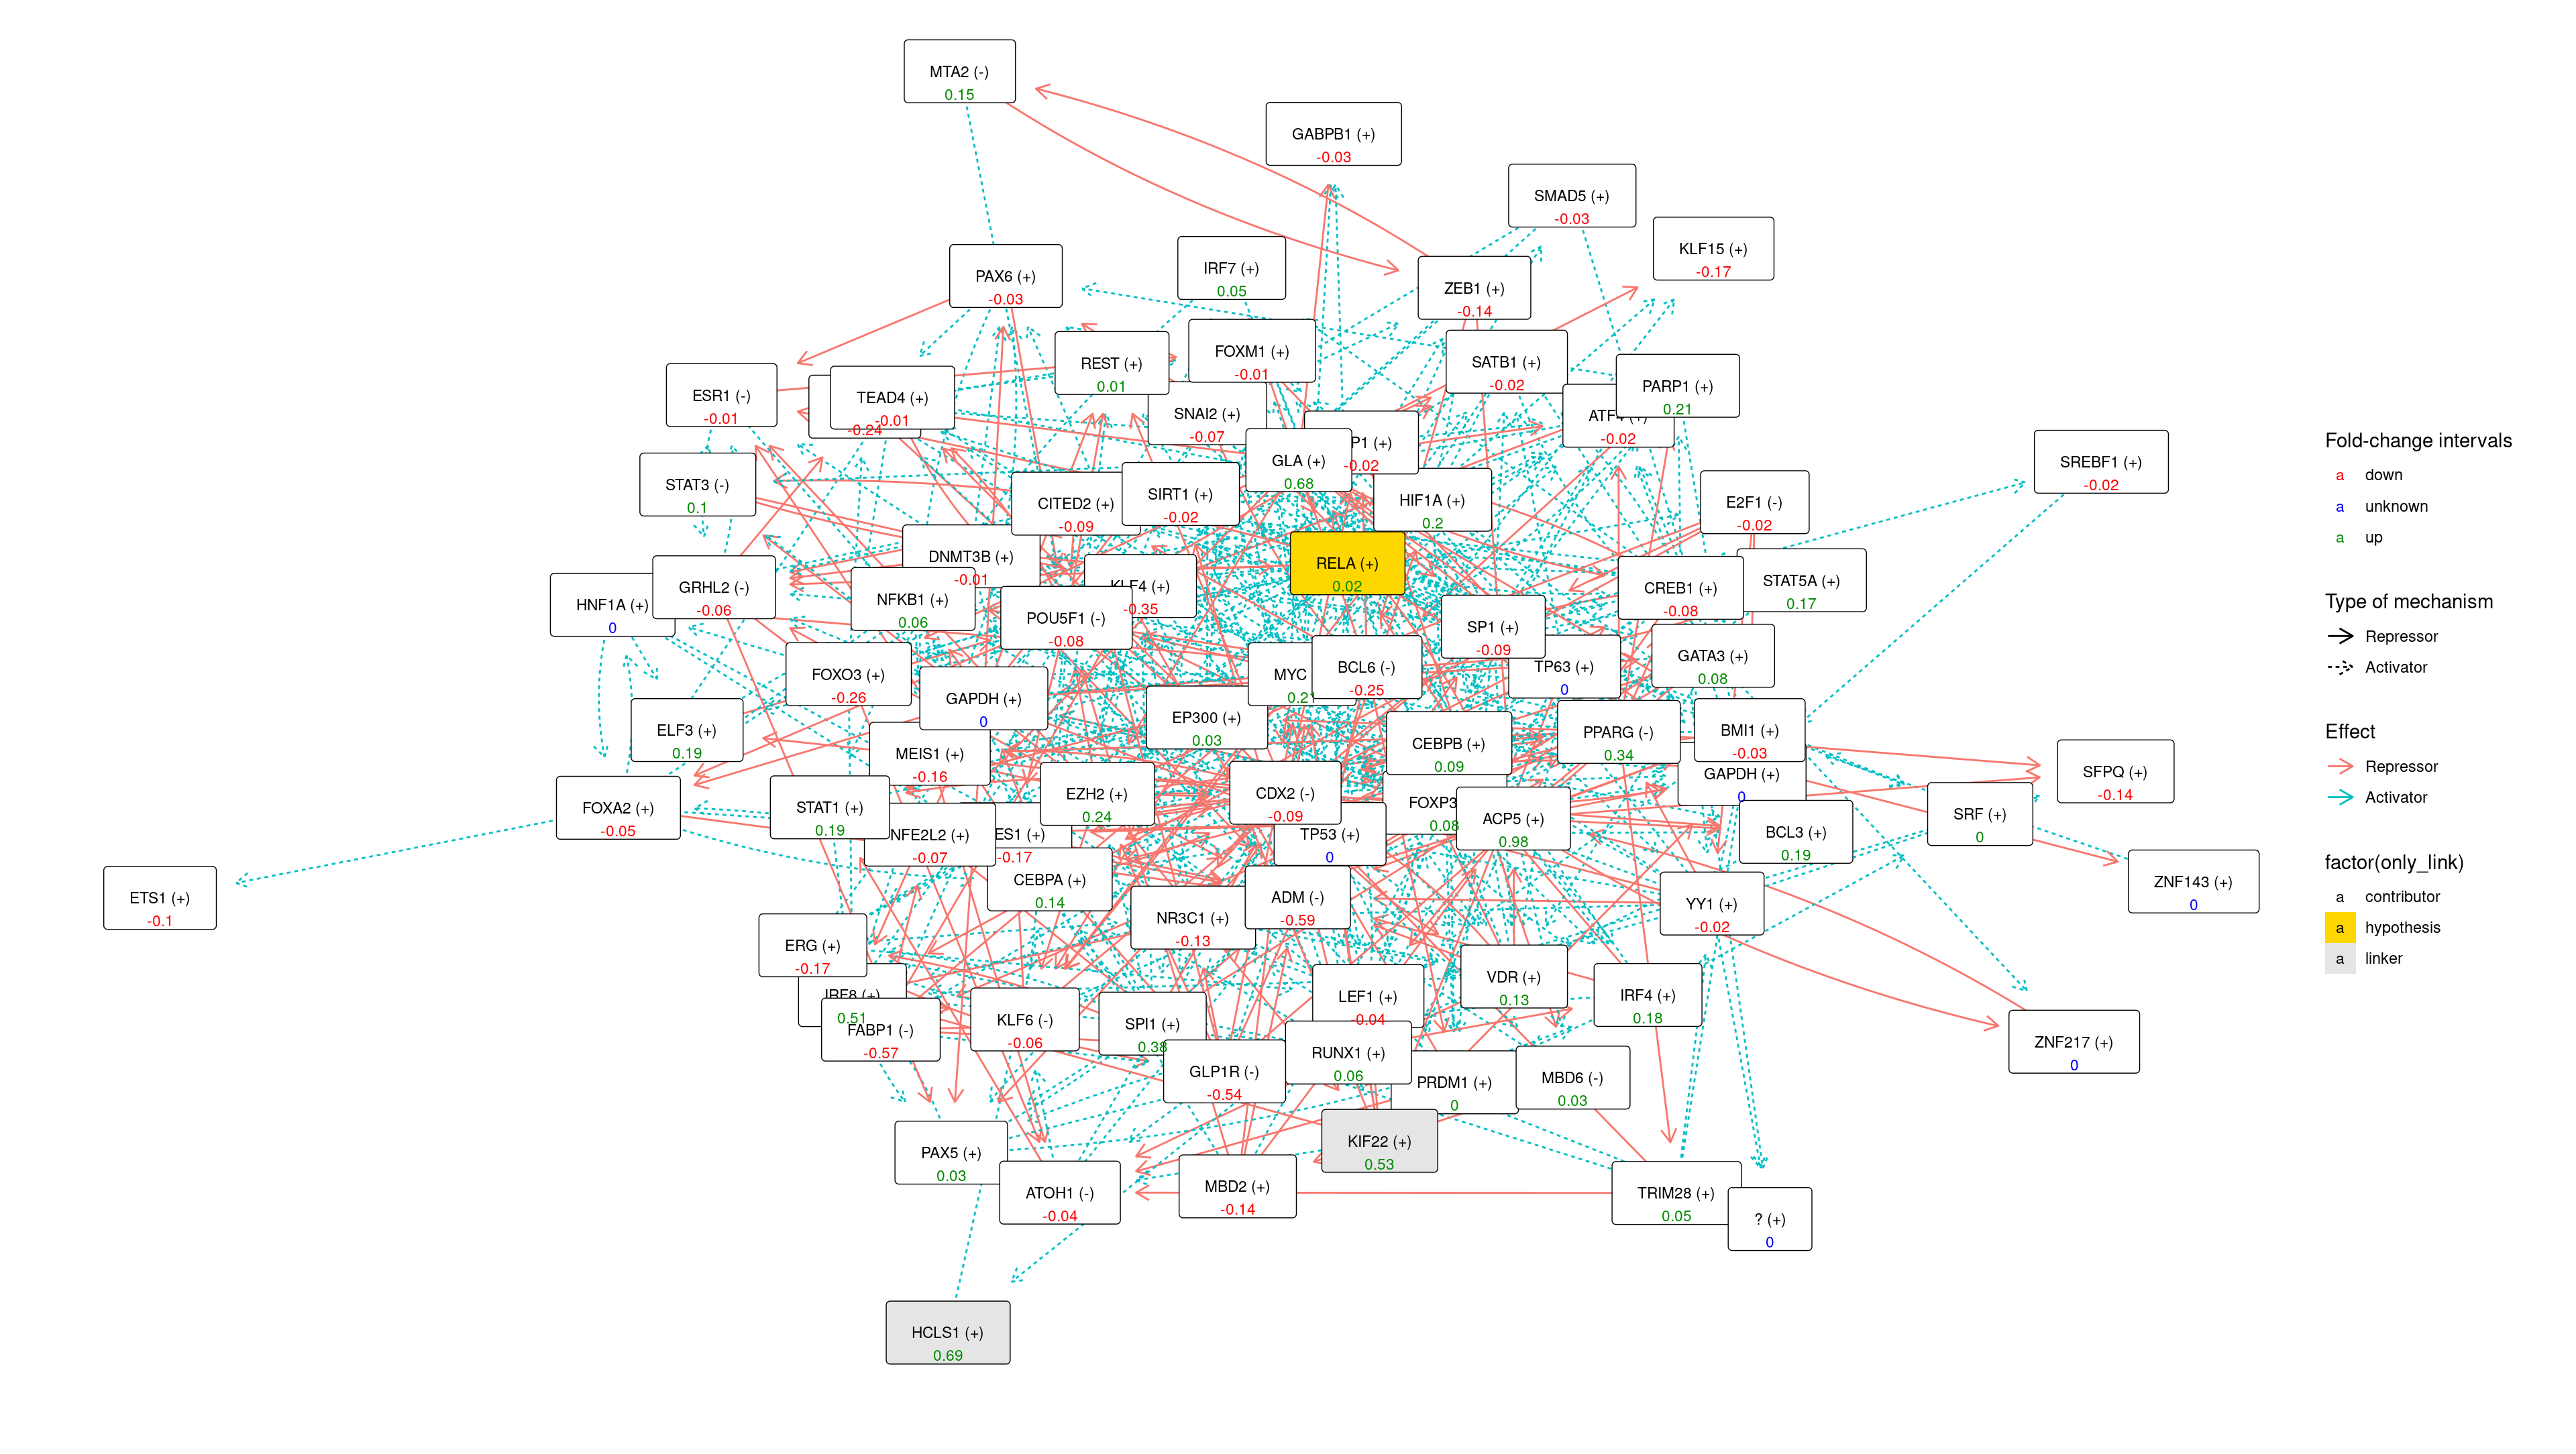
\includegraphics[width=\textwidth, height=\textheight, keepaspectratio]{Major Thesis/figures/iut/graph/CESS4m50-RELA.png}
            \caption{CESS 4m contrast}
            \label{img:prev-smoke}
    \end{subfigure}
    \hfill
    \begin{subfigure}{0.3\linewidth}
        \centering
        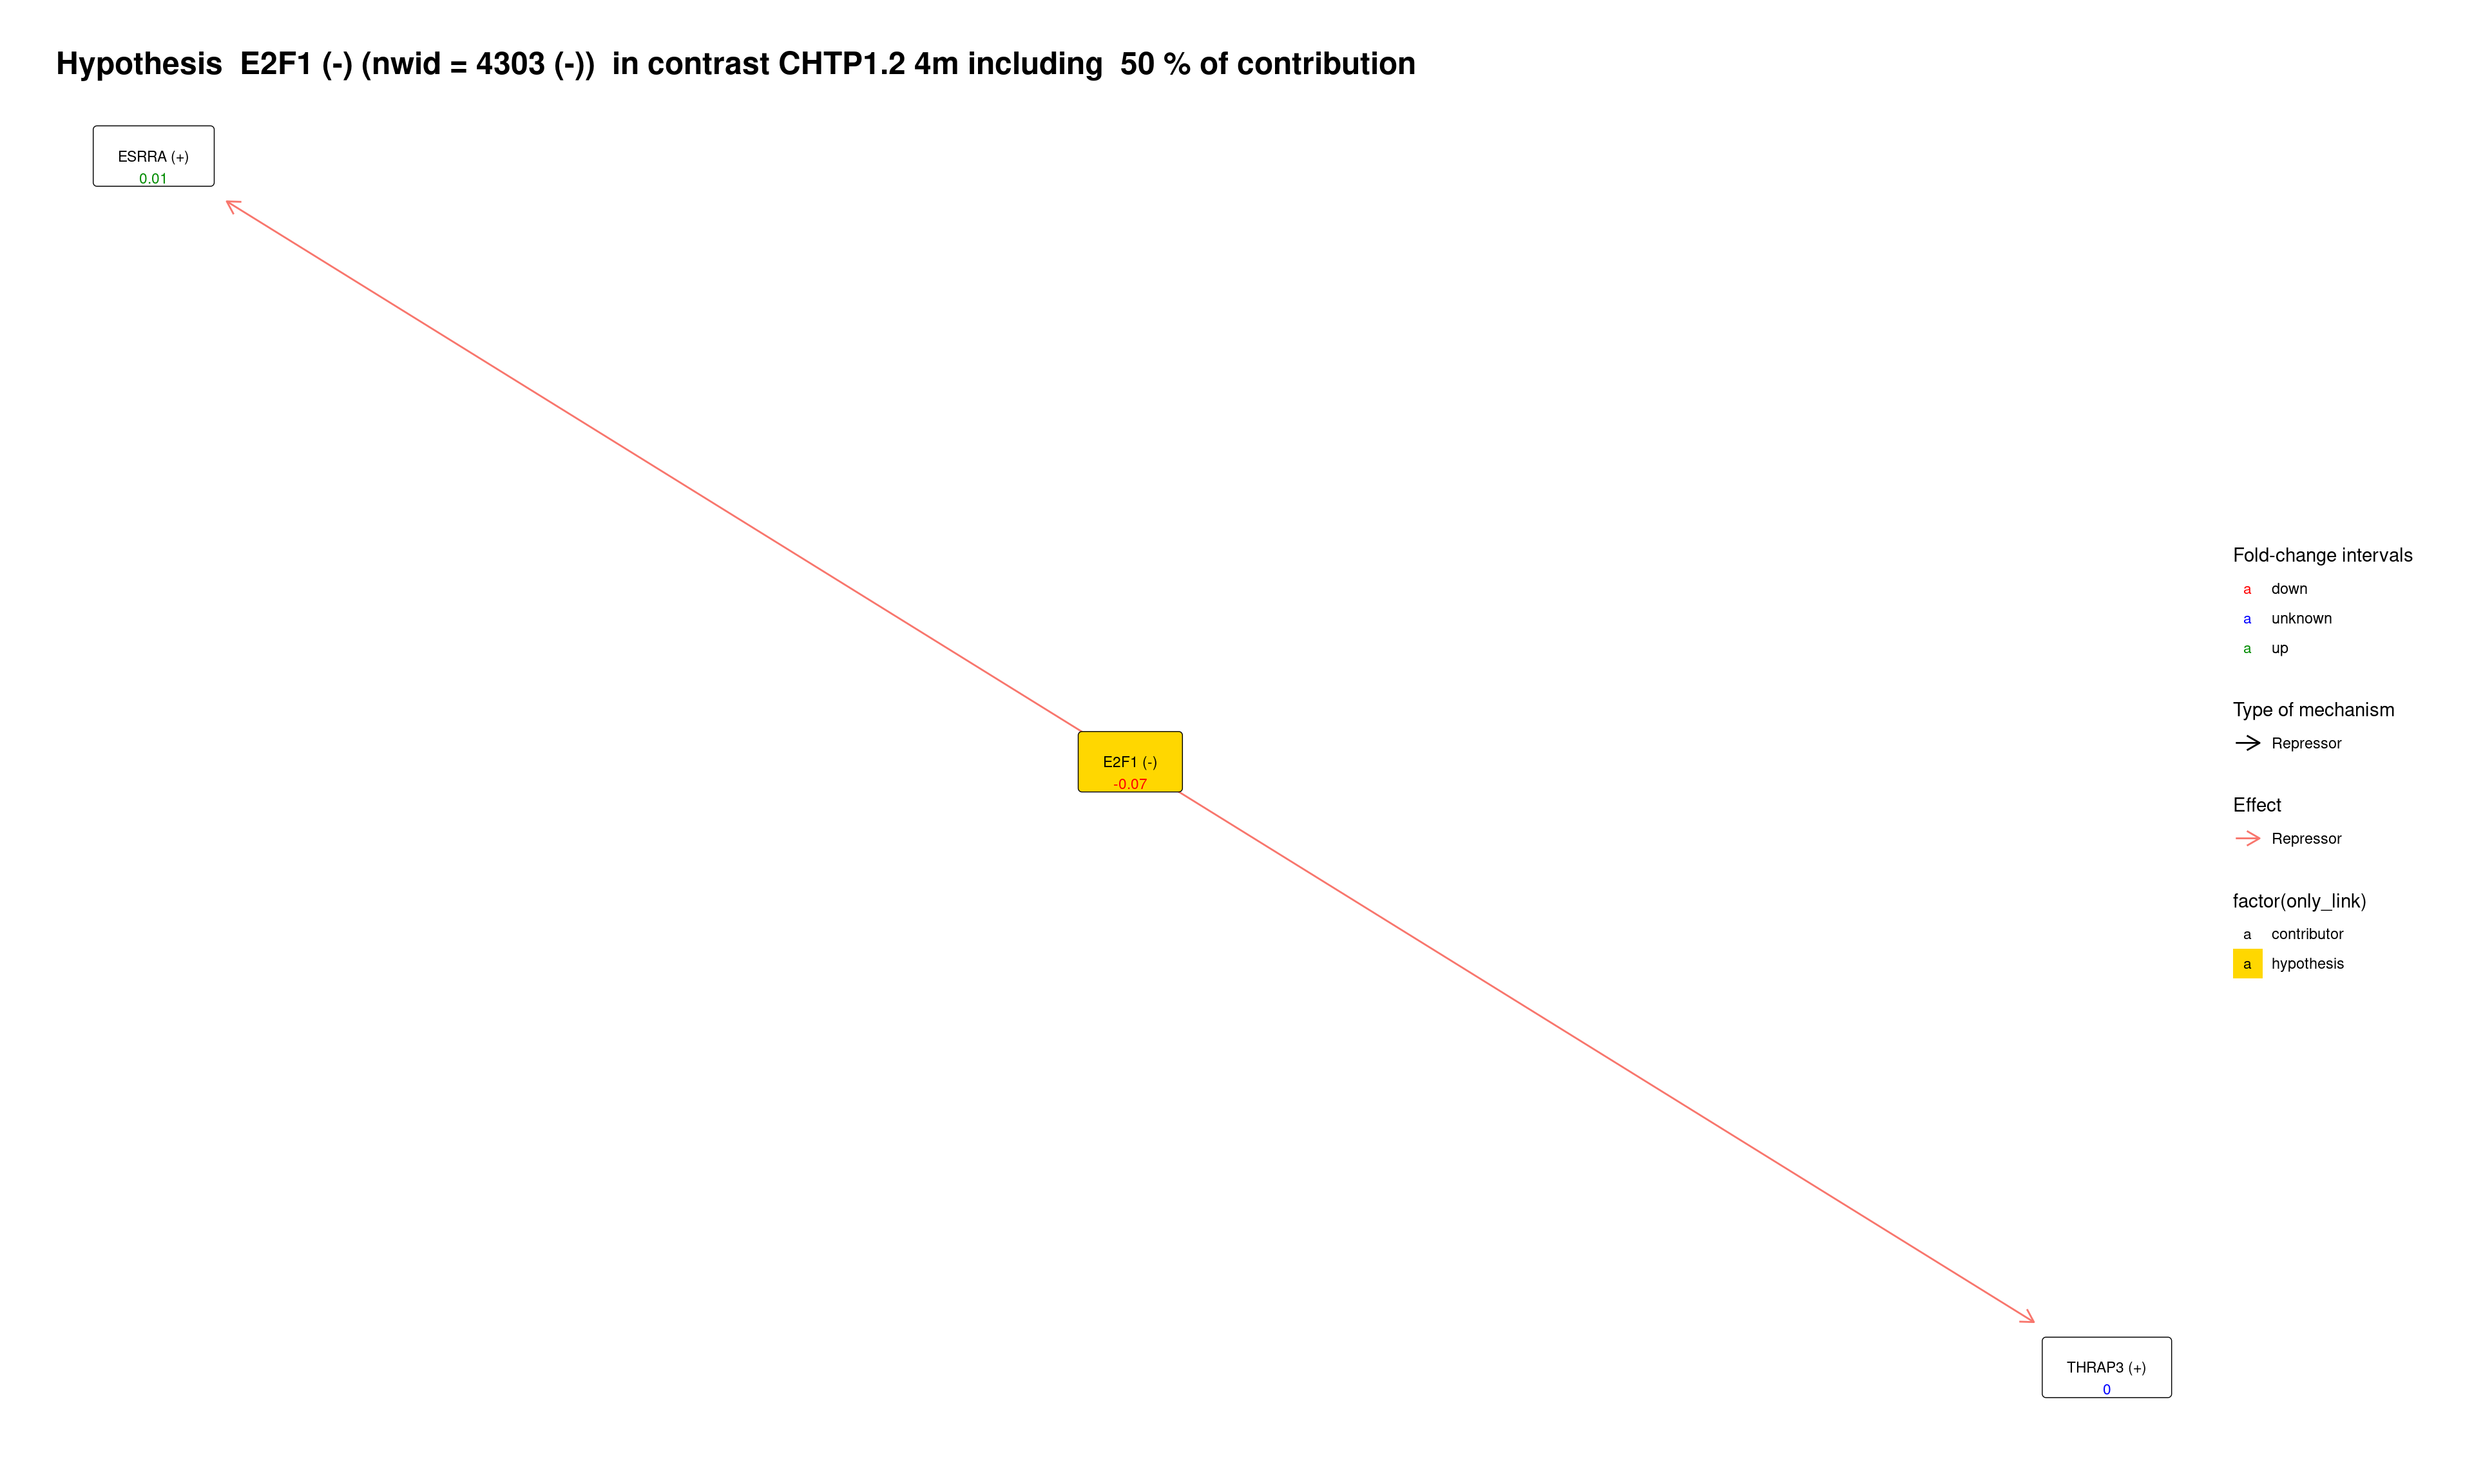
\includegraphics[width=\textwidth, height=\textheight, keepaspectratio]{Major Thesis/figures/iut/graph/CHTP4m-E2F1.png}
            \caption{CHTP 4m contrast}
            \label{img:non-smoke}
    \end{subfigure}
    
    \caption{Node density comparison at 50\% contribution among (a) smoke contrast, (b) smoked past and (c) aerosol products under same exposure time.}
    \label{fig:compare-density}
\end{figure}

As for an overview study among contrasts, we now switch to Figure \ref{fig:heatmap-overview} for the top ranked DE genes ranking displayed on a heat-map-like mode.

\begin{figure}
    \centering
    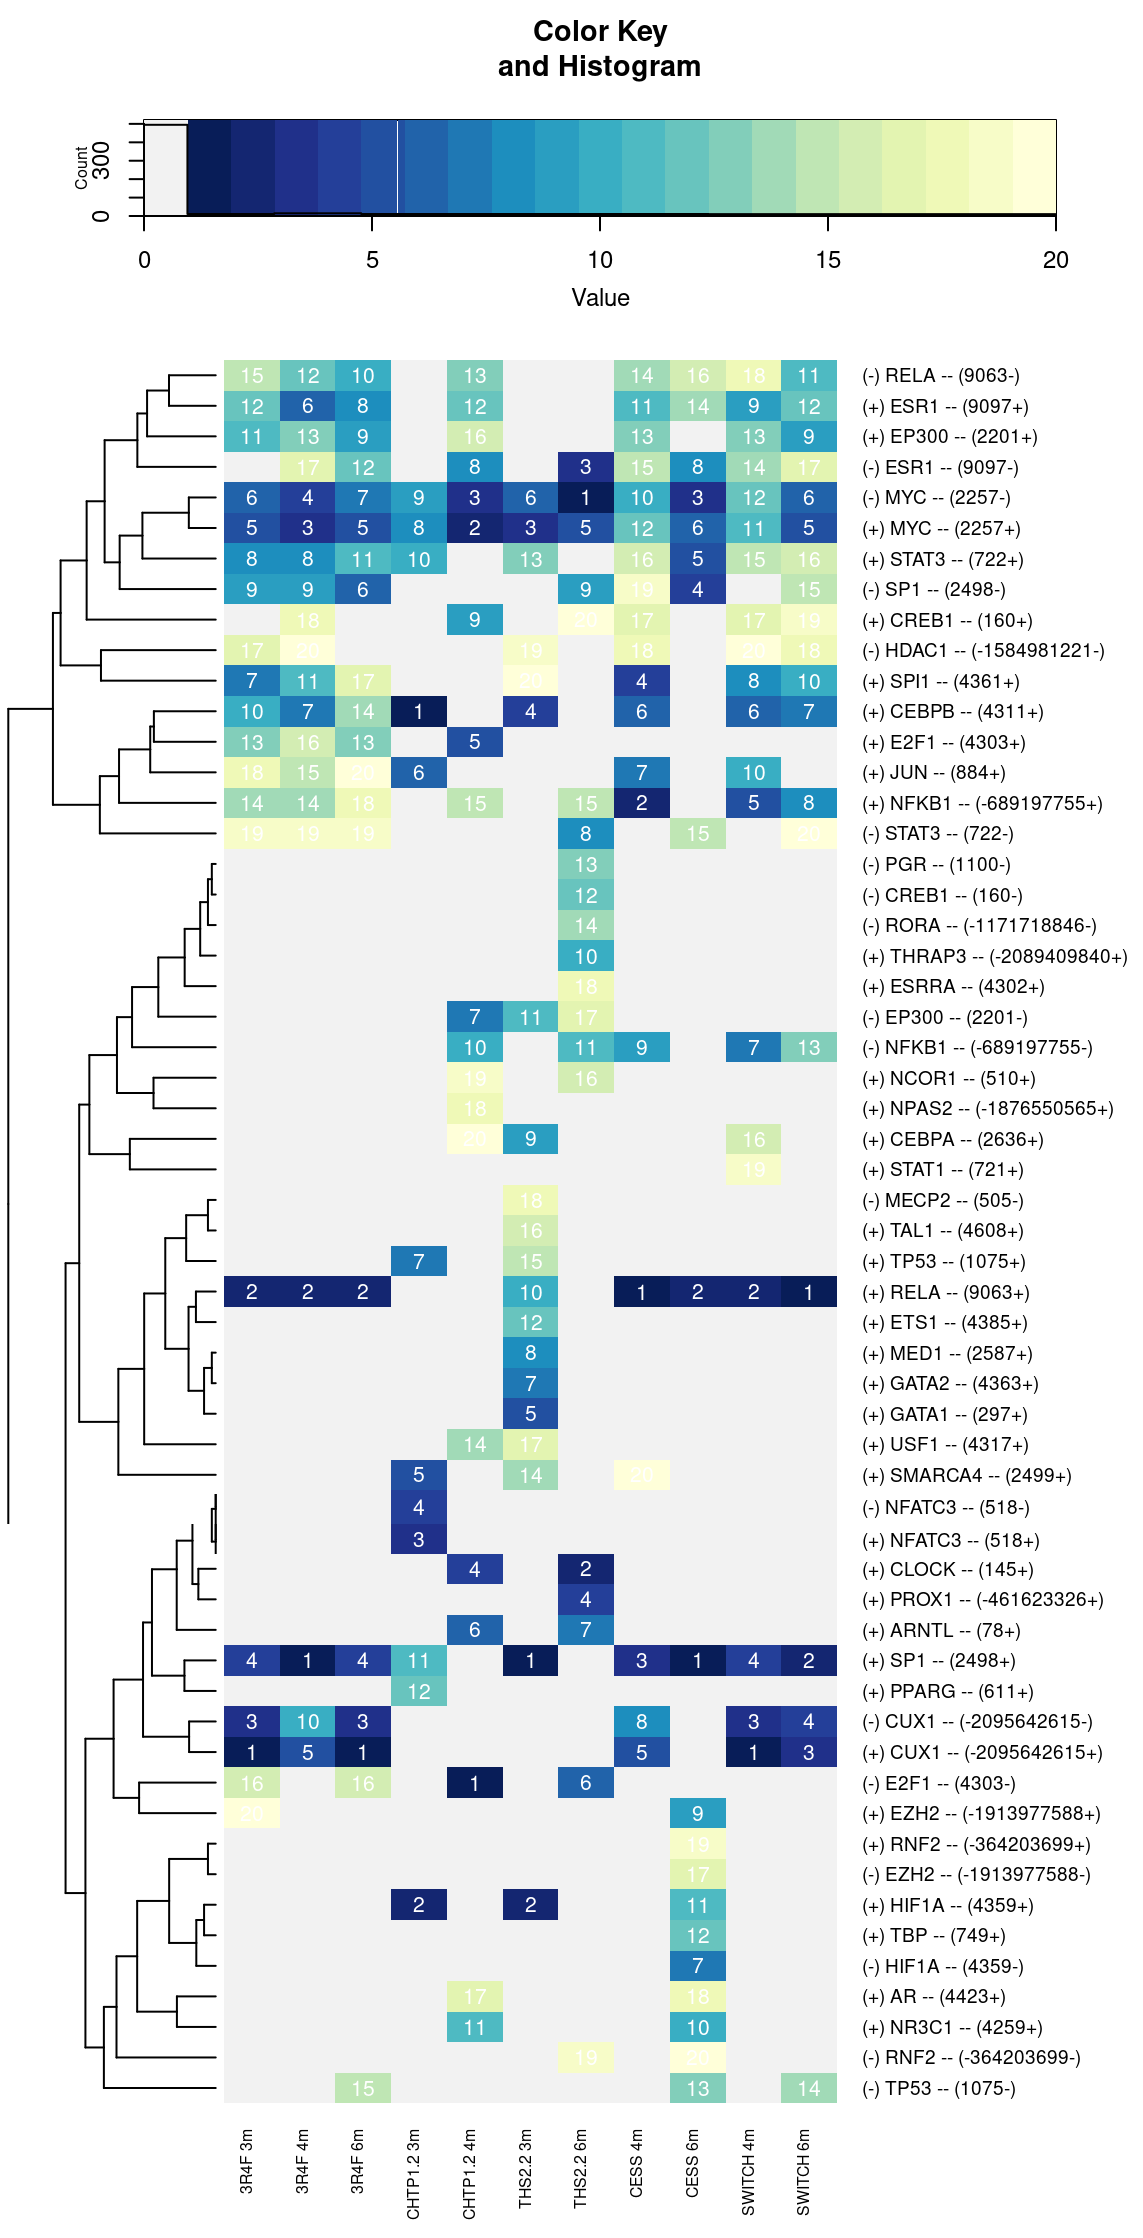
\includegraphics[width=\textwidth, height=\textheight, keepaspectratio]{Major Thesis/figures/iut/heat/heatmap-contrasts.png}
    \caption{Particular heat map built on 3R4F 4m contrast. Discriminates outliers (left) from cases (right) taken into consideration for subnetwork calculation.}
    \label{fig:heatmap-overview}
\end{figure}

Predictions of contrasts 3R4F, SWITCH and CESS —--in all their timepoints—-- were expected to have a similar signature, since they experiment has been performed on subjects which have been exposed to cigarette smoke (CS). As s subgroup, SWITCH and CESS also hold the relation of quitting CS exposition at a set time, therefore, their result match also makes sense.
\\

Instability of results can likely be also explained by overall low response to THS2.2 expose. The discrepancy of top ranked genes, however, lays in the detection, not in the rank value, as genes ranked in a first position for a lower exposure time (3 months) have not even entered the top ranked genes in the longer exposure (6 months).
\\

As seen, SigNet delivers a broader view of the candidates as we can see the full network ranked. MARINa suffers hypotheses loss at the enrichment step due to its GSEA and shadowing filtering methods. As a result, the outcome remains incomplete for in-depth exploration, since only a few top predictions are returned.
\\

\begin{table}[h]
\centering
\begin{tabular}{|l|l|l|l|}
\hline
gene\_id & symbol & GO id      & term                           \\ \hline
1523     & CUX1   & GO:0016020 & membrane                       \\ \hline
1523     & CUX1   & GO:0016021 & integral component of membrane \\ \hline
1523     & CUX1   & GO:0005794 & Golgi aparatus                 \\ \hline
…        & …      & …          & …                              \\ \hline
4609     & MYC    & GO:0005634 & nucleus                        \\ \hline
\end{tabular}
\caption{Top N ranked items selected alongside their retrieved GO term via BiomaRt.}
\label{tbl:goterms}
\end{table}

When joined together using an overlap (Figure img:comparisonSM), we see there’s a slight consensus among both, i.e. top cases (top 5\% of results) from SigNet are also present in MARINa’s result set. Due to this support, we present intersected results as first candidates to be further explored with interaction graphs.
\\

Due to previously (lab) User specified needs, GO terms for the top results have also been added to the selected results (Table 1).

\subsubsection{DES-nA Component}
[Indicate time-points + differences]

In this case, the graphs have been generated de novo while using a reference for interactions. New graph results might appear, which would do not perfectly match known pathways, nor diverge largely from the curated ground truth. These are based entirely on the input data and serve us to pinpoint dissimilarities in particular individuals.
\\

A second overview represents via a heat map the fold-change of each of the nodes present in a certain subnetwork, across all the contrasts that have been used to calculate said subnetwork. 
\\

Figure img:DESNA-heatmaps helps on boundary setting by displaying an overview of the cases. The percentage of cases which are dysregulated can be seen at first sight which, in turn, can be used to colour graphs as Figure img:DESNA-graphs. 
\\

\begin{figure}
    \centering
    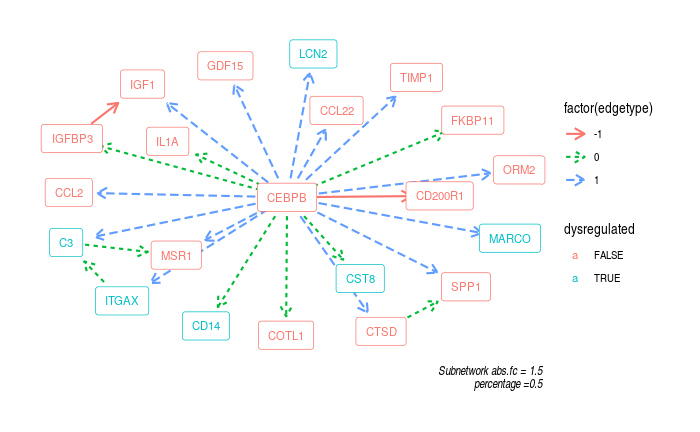
\includegraphics[width=\textwidth]{Major Thesis/figures/desna/desna-network.png}
    \caption{Network built on [contrast] DEG data. Fold-change threshold to consider expression as DEG = 1.5. A node is considered as dysregulated if 0.5 (50\%) of the cases are DE, i.e. FC >= 1.5}
    \label{fig:desna-network}
\end{figure}

Visualization and further inspection has been designed based on some UX principles. In this case, mainly using colour scales and matching input’s original names instead of using network names. An interactive of this graphs has been considered unnecessary due to their simplicity.

\subsection{Suitability based on accuracy}
Since the previous section agrees on the fact all the algorithms are suitable for biological information extension and dispose of the same properties when it comes to straightforward interpretation, the following points aim to ease the task of choosing which to method to deliver per component as the most suitable in terms of visualisation and accuracy.
We must keep in mind IUT and DES-nA are not comparable in terms of accuracy metrics, as their approaches and benchmarking systems differ. Besides we miss DES-nA’s Benchmark Core and, therefore, accuracy results.

\subsubsection{IUT Component}
During assessment, both minimum start nodes (msn) and FDR-corrected p-value (adj.pvalue) parameters act as filters for the input nodes in SigNet’s run. However, based on the benchmarking we conclude only adj.pvalue interferes in the prediction accuracy, while the minimum start nodes amount does not. This effect happens because the adj.p.value filters down the nodes only, reducing the amount of elements to forward to the main algorithm. A value of 0.05 is used, both due to literature recommendations and due to parameter tuning performed at the B Core.
\\

\begin{table}[]
\centering
\resizebox{\textwidth}{!}{%
\begin{tabular}{|c|c|c|c|c|}
\hline
\multicolumn{1}{|l|}{}                                         & \cellcolor[HTML]{0C61AB}{\color[HTML]{FFFFFF} Output} & \cellcolor[HTML]{4184C0}{\color[HTML]{FFFFFF} Accuracy} & \cellcolor[HTML]{0C61AB}{\color[HTML]{FFFFFF} Method} & \cellcolor[HTML]{4184C0}{\color[HTML]{FFFFFF} Results/Input} \\ \hline
\rowcolor[HTML]{F2F2F2} 
\cellcolor[HTML]{52CB98}{\color[HTML]{FFFFFF} \textbf{SigNet}} & Full causal network ranked                            & $\sim$25 \% in first the 2000. $\sim$80\% overall       & Causal graph inference                                & 100 \%                                                       \\ \hline
\cellcolor[HTML]{E53265}{\color[HTML]{FFFFFF} \textbf{MARINa}} & Top GSEA nodes ranked                                 & $\sim$5 \% overall                                      & GSEA + Shadow                                         & $\sim$0.05\%                                                 \\ \hline
\end{tabular}%
}
\end{table}

MARINa results should not be directly compared on the same scale as SigNet’s due to the result set. MARINa only returns the top-ranked hypothesis which passes all the filters, while SigNet ranks the full (cropped by the filters of the Format Core) network. A standard run results in a rank size of 10 for the former and 46.360 for the latter, out of a total 57.606 input. The accuracy scores are rescaled to the match the total size of the output.
The benchmark is run on both algorithms using the same N test cases. The main accuracy score relies on presence of the real target (extracted from TTD and CMAP2) in the hypothesis set from the result (from the algorithms), i.e. if the target has been predicted. Results can be seen in Figure img:SigNetMARINaBench
\\

The low scoring of MARINa is a consequence of the accuracy of the methods: The top-ranked hypothesis contain at most a 2 out of 10 targets match. In turn, the average score among all N test cases drops below 5\% accuracy.

\subsubsection{DES-nA Component}
Since the DES-nA component could not be assessed using a gold standard we skip this section and forward a conclusion based on visualization properties straight to the Discussion.